\documentclass[12pt,letterpaper]{article}

\newenvironment{proof}{\noindent{\bf Proof:}}{\qed\bigskip}

\newtheorem{theorem}{Theorem}
\newtheorem{corollary}{Corollary}
\newtheorem{lemma}{Lemma} 
\newtheorem{claim}{Claim}
\newtheorem{fact}{Fact}
\newtheorem{definition}{Definition}
\newtheorem{assumption}{Assumption}
\newtheorem{observation}{Observation}
\newtheorem{example}{Example}
\newcommand{\qed}{\rule{7pt}{7pt}}

\newcommand{\assignment}[4]{
\thispagestyle{plain} 
\newpage
\setcounter{page}{1}
\noindent
\begin{center}
\framebox{ \vbox{ \hbox to 6.28in
{\bf CS446: Machine Learning \hfill #1}
\vspace{4mm}
\hbox to 6.28in
{\hspace{2.5in}\large\mbox{Problem Set #2}}
\vspace{4mm}
\hbox to 6.28in
{{\it Handed Out: #3 \hfill Due: #4}}
}}
\end{center}
}

\newcommand{\solution}[4]{
\thispagestyle{plain} 
\newpage
\setcounter{page}{1}
\noindent
\begin{center}
\framebox{ \vbox{ \hbox to 6.28in
{\bf CS446: Machine Learning \hfill #4}
\vspace{4mm}
\hbox to 6.28in
{\hspace{2.5in}\large\mbox{Problem Set #3}}
\vspace{4mm}
\hbox to 6.28in
{#1 \hfill {\it Handed In: #2}}
}}
\end{center}
\markright{#1}
}

\newenvironment{algorithm}
{\begin{center}
\begin{tabular}{|l|}
\hline
\begin{minipage}{1in}
\begin{tabbing}
\quad\=\qquad\=\qquad\=\qquad\=\qquad\=\qquad\=\qquad\=\kill}
{\end{tabbing}
\end{minipage} \\
\hline
\end{tabular}
\end{center}}

\def\Comment#1{\textsf{\textsl{$\langle\!\langle$#1\/$\rangle\!\rangle$}}}


\usepackage{epstopdf}
\usepackage{graphicx,amssymb,amsmath}
\oddsidemargin 0in
%\evensidemargin 0in
\textwidth 6.5in
%\topmargin -0.5in
\textheight 9.0in

\begin{document}

\solution{Chen Zhang}{9/16/2014}{1}{Fall 2014}
% Fill in the above, for example, as follows:
% \solution{Joe Smith}{\today}{1}{Fall 2012}

\pagestyle{myheadings}  % Leave this command alone

%\begin{enumerate}
%\item Answer to problem 1
%\item Answer to problem 2
%\item Answer to problem 3
%\end{enumerate}
\section{Problem 1}
\subsection{Algorithm}
Loop over the training data from 1 to m, call the current data i
\\ \indent if the i-th label is positive
\\ \indent \indent Don't do anything
\\ \indent if the i-th label is negative
\\ \indent \indent take negation of the x vector (E.g if $x=[1\quad1\quad0\quad1]$, the negation is $\hat{x}=[0\quad0\quad1\quad0]$). 
\\ \indent \indent use $\hat{x}$ as a start , set $p=i$ and break out of the loop
\\Loop over the training data from p to m, call the current data i
\\ \indent if the i-th label is positive
\\ \indent \indent Don't do anything
\\ \indent if the i-th label is negative
\\ \indent \indent remove the duplicate element between $\hat{x}$ and $x_i$ and make the resulting quantity the 
\\ \indent \indent new $\hat{x}$(E.g if $\hat{x}$ contains $x_1=1\quad x_3=0\quad x_8=1 \quad x_{12}=0$ and a data with negative \\ \indent \indent label contains $x_1=1 \quad x_3=0$, then the resulting quantity is $x_8=1 \quad x_{12}=0$). 
\\ If the final $\hat{x}$ is not empty, then $\hat{x}$ is a valid disjunction.
\\ If the final $\hat{x}$ is empty
\\ \indent If all the training data have positive label
\\ \indent \indent \textbf{Always Positive} is a valid disjunction for the training data.
\\ \indent If all the training data have negative label 
\\ \indent \indent \textbf{Always Negative} is a valid disjunction for the training data.
\\ \indent If the training data have both positive label and negative label 
\\ \indent \indent There is no valid disjunction for this data set

\subsection{Prove correctness}
If there is no negative training data in the set, we will have a \textbf{Always Positive} as the disjunction, which is obviously true with the training data.
\\If there is at least one negative training data, we know that by taking the negation of every variable in the data, the true disjunction ( if there is any ) is definitely a subset of this resulting disjunction. Then by removing the duplicate element, because of the nature of disjunction, we are ruling out the impossible, and the true disjunction will always be a subset of the resulting disjunction. In that sense, if there is a true disjunction, it will be a subset of the resulting disjunction. Thus the training data with positive label will always have the correct prediction. Since the resulting disjunction is obtained by removing duplicate elements of data with negative label, it will always have correct prediction as well. Thus the algorithm will label the training data exactly as it should be.   

\subsection{Analyze Complexity}
Inside each loop, if the training data has positive label, we don't do anything. So we can assume the worst case where all the data have negative label. 
\\In this case inside each loop we are either taking negation or comparing and removing element from a total of n elements. Thus the maximum time needed inside one loop is n. 
\\Because we are looping over m training data. Thus the maximum is O(mn), which is polynomial in terms of training data and number of variables. 

\subsection{Testing Cases}
(A)When the resulting disjunction is \textbf{Always Positive}( This would be the case when all the training data have positive label). Clearly if the new data have negative label, this is not correct. If new data has positive label, this is correct.
\\(B)The resulting disjunction is \textbf{Always Negative}. Clearly if the new data have positive label, this is not correct. If new data has negative label, this is correct.
\\(C)The resulting disjunction is not empty. Because the algorithm is based on canceling the duplicate elements of the data with negative label, the true disjunction is a subset of the resulting disjunction. With this being the case, the testing data which should have a positive label will be predicted correctly. However, a testing data which should have a negative label have a potential of being predicted incorrectly, when it does not belong to the true disjunction but belongs to the resulting disjunction

\section{Problem 2}
\subsection{Point and HyperPlane}
Suppose $x_1$ is one point at the hyper plane. The distance between point $x_0$ is the projection of vector $\vec{x}_0-\vec{x}_1$ onto the normal vector of the hyper plane ($\vec{w}^T\vec{x}_1+\theta=0$). Thus we have the equation as 
\begin{equation*}
D_1=|\frac{(\vec{x}_0-\vec{x}_1)*\vec{w}}{|\vec{w}|}|=|\frac{\vec{x}_0*\vec{w}-\vec{x}_1*\vec{w}}{|\vec{w}|}|=\frac{|\vec{x}_0*\vec{w}+\theta|}{|\vec{w}|}
\end{equation*}

\subsection{HyperPlane and HyperPlane}
Since these two hyper planes have the same $\vec{w}$, we know that these two hyper planes are parallel to each other. Thus the distance between two hyper planes are the distance between a point on hyper plane A to hyper plane B ($\vec{w}^T\vec{x}_1+\theta_1=0$) and ($\vec{w}^T\vec{x}_2+\theta_2=0$). Thus using the result above we have 
\begin{equation*}
D_2=|\frac{(\vec{x}_2-\vec{x}_1)*\vec{w}}{|\vec{w}|}|=|\frac{\vec{x}_2*\vec{w}-\vec{x}_1*\vec{w}}{|\vec{w}|}|=\frac{|\vec{x}_2*\vec{w}+\theta_1|}{|\vec{w}|}=\frac{|\theta_1+\theta_2|}{|\vec{w}|}
\end{equation*}

\section{Problem 3}
\subsection{Part a}
\subsubsection{Proof}
\noindent If two datasets are linear separable, by analysing the closest point to the hyperplane, we could see that there exists a $\vec{a}$ and $b$ such that $\vec{a}^tX_i-b\geq1$ for the first dataset and $\vec{a}^tX_i-b\leq-1$ for the second dataset ( If not, by proper scaling of $\vec{a}$, we will have these two planes. ). See Fig 1. Then if we give the first class a tag $y_i=1$ and the second class a tag $y_i=-1$, we have the equation $y_i(\vec{a}^T\vec{x}_i+b)\geq 1$. By using $\vec{a}=\vec{w}$ and $b=\theta$, we have $y_i(\vec{w}^T\vec{x}_i+\theta)\geq 1$. Thus that the optimal solution of $\delta$ for the following equation is $\delta=0$.
\begin{eqnarray*}
	\min_{\vec{w}, \theta, \delta} & & \delta  \label{eq:lin_prog_discriminant_obj}\\
	\textrm{subject to } & & y_i(\vec{w}^T \vec{x_i} + \theta) \geq 1 - \delta, \qquad \forall (\vec{x_i},y_i) \in D  \label{eq:lin_prog_discriminant_constraint}\\
	& & \delta \geq 0  \label{eq:lin_prog_discriminant_bound}
\end{eqnarray*}

\noindent On the other hand, if the above equation is satisfied with optimal solution $\delta=0$, then we have $y_i(\vec{a}^T\vec{x}_i+b)\geq 1$. Expand this equation, if $y_i=1$ then $\vec{a}^T\vec{x}_i+b\geq 1$. If $y_i=-1$ then $\vec{a}^T\vec{x}_i+b\leq -1$. This satisfies the definition for linear separability, meaning the two datasets are linear separable.
\begin{figure}[h!]
	\centering
	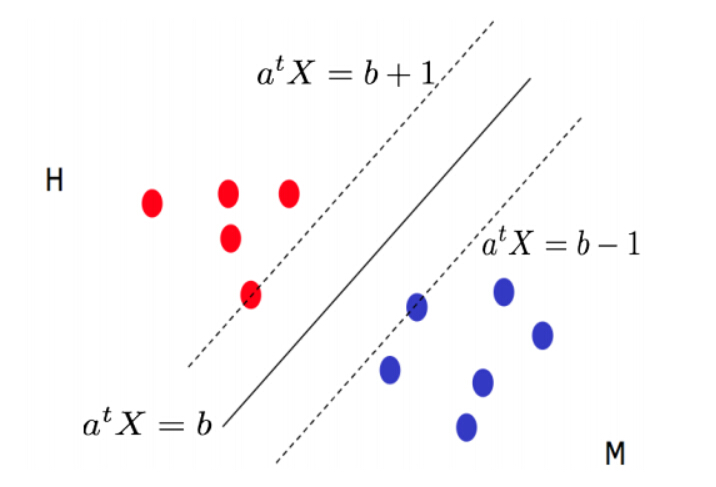
\includegraphics[width=0.8\textwidth]{LinearSeparable}
	\caption{Two linear separable dataset. Courtesy: Barnabas Poczos, Carnegie Mellon University}
\end{figure}

\subsubsection{Trivial Solution}
\begin{eqnarray*}
    	%      \min_{\vec{w},\theta,\delta} & & \delta  \\
    	\min_{\vec{w}, \theta, \delta} & & \delta  \\
    	\textrm{subject to } & & y_i(\vec{w}^T \vec{x_i} + \theta) \geq - \delta, \qquad \forall (x_i,y_i) \in D \\
    	&& \delta \geq 0  \\
\end{eqnarray*}
In the above expression, an optimal solution would be $\delta=0$. But this solution is trivial because even if this solution is satisfied, it is not guaranteed that the dataset is linear separable ( and vice versa ). 

\noindent Assume that we have points that satisfy $\vec{w}^T\vec{x}_i+\theta=0$. Then whatever tag these points have ($y_i=1$ or $y_i=-1$), it still satisfies $ y_i(\vec{w}^T \vec{x_i} + \theta) \geq - \delta$ at the optimal solution $\delta=0$. Thus on the plane defined by $\vec{w}^T\vec{x}_i+\theta=0$, we have both positive tag points and negative tag points, meaning that they are not linearly separable. Thus that this solution is trivial and this is why we choose the previous formulation rather than this one.  
\subsubsection{Hand Calculation}
Expanding the linear program, we have the following equations:
\begin{equation*}
\vec{w}^t\begin{bmatrix}
1& 1& 1 \ldots & 1 & 1 & 1
\end{bmatrix}^T_{1\times n}+\theta\geq 1-\delta
\end{equation*}
\begin{equation*}
\vec{w}^t\begin{bmatrix}
-1& -1& -1 \ldots & -1 & -1 & -1
\end{bmatrix}^T_{1\times n}+\theta\leq \delta-1
\end{equation*}
\noindent Note that this case we only have two points of different tags, thus the dataset is for sure linear separable. This means the optimal solution could reach $\delta=0$.  Use this fact and multiply -1 at the left hand side and right hand side of the equation and expand the vector multiplication, we have the following equation:
\begin{equation}
w_1+w_2+w_3+\ldots+w_{n-1}+w_n+\theta\geq 1
\end{equation}
\begin{equation}
w_1+w_2+w_3+\ldots+w_{n-1}+w_n-\theta\geq 1
\end{equation}
Thus any $\vec{w}$ and $\theta$  that satisfies equation (1) and (2) could be the separating plane.

\subsection{Part b}
\subsubsection{Writing LP}
The starting linear program we have is:
\begin{eqnarray*}
\min_{\vec{w}, \theta, \delta} & & \delta  \label{eq:lin_prog_discriminant_obj}\\
\textrm{subject to } & & y_i(\vec{w}^T \vec{x_i} + \theta) \geq 1 - \delta, \qquad \forall (\vec{x_i},y_i) \in D  \label{eq:lin_prog_discriminant_constraint}\\
& & \delta \geq 0  \label{eq:lin_prog_discriminant_bound}
\end{eqnarray*}
where $D$ is the data set of all training examples. Expand the set of equation we have 
\begin{eqnarray*}
\min_{\vec{w}, \theta, \delta} & & \delta  \label{eq:lin_prog_discriminant_obj}\\
\textrm{subject to } & & \vec{w}^T \vec{x_i}y_i + y_i\theta + \delta \geq 1, \qquad \forall (\vec{x_i},y_i) \in D  \label{eq:lin_prog_discriminant_constraint}\\
& & \delta \geq 0  \label{eq:lin_prog_discriminant_bound}
\end{eqnarray*}

\noindent Construct the vectors $\vec{t}^T =
\begin{bmatrix}
w_1 & w_2 & w_3 \ldots & w_n & \theta & \delta
\end{bmatrix}_{1\times(n+2)}$, $\vec{c}^T= \begin{bmatrix}
0 & 0 & 0 \ldots & 0 & 0 & 1
\end{bmatrix}_{1\times(n+2)}$ $\vec{b}^T= \begin{bmatrix}
1 & 1 & 1 \ldots & 1 & 1 & 1
\end{bmatrix}_{1\times m}$, $A_{m,n+2} =
\begin{pmatrix}
x_{1,1}y_1 & x_{1,2}y_1 & \cdots & x_{1,n}y_1 & y_1 & 1 \\
x_{2,1}y_2 & x_{2,2}y_2 & \cdots & x_{2,n}y_2 & y_2 & 1\\
\vdots  & \vdots  & \ddots & \vdots & \vdots & \vdots \\
x_{m,1}y_m & x_{m,2}y_m & \cdots & x_{m,n}y_m & y_m & 1
\end{pmatrix}_{m\times (n+2)}$

\noindent This way the original starting linear program could be written in a standard linear program as:
\begin{eqnarray*}
\min_{\vec{w}, \theta, \delta} & & z(\vec{t})=\vec{c}^T\vec{t}  \label{eq:lin_prog_discriminant_obj}\\
\textrm{subject to } & & A\vec{t}\geq\vec{b}, \qquad \forall (\vec{x_i},y_i) \in D  \label{eq:lin_prog_discriminant_constraint}\\
& & \delta \geq 0  \label{eq:lin_prog_discriminant_bound}
\end{eqnarray*}

\subsubsection{Learning Conjunctions}

\begin{figure}[h!]
	\centering
	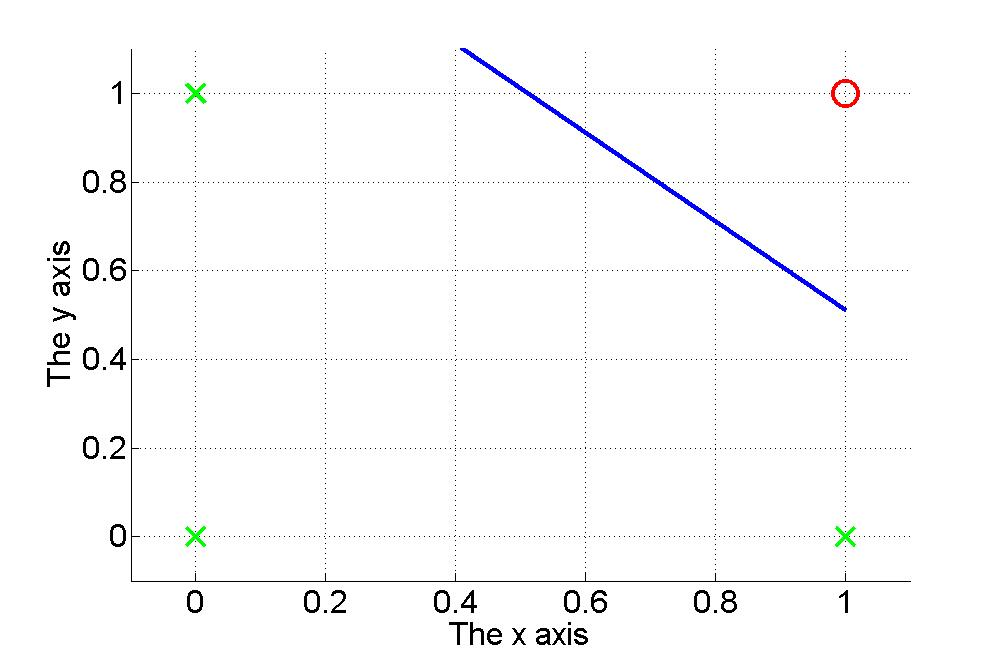
\includegraphics[width=0.8\textwidth]{learnConjunctions}
	\caption{Part 1 of Learning Conjunctions}
\end{figure}
\noindent For the first part, please refer to Fig 1.

\noindent For the second part, the linear discriminant separator returned is:

\noindent $\vec{w}^T =
\begin{bmatrix}
2.6931 & -2.6607 & 0.9445 & 185.6576 & 1.1473 & -1.7095 & -3.3430 & -187.8564 & 0.2931 & -9.0398
\end{bmatrix}$, $\theta=-87.6922$, $\delta=2.2374\times 10^{-11}$.
From the separator we know that the conjunction is $(x_4 \vee \neg x_8 )$. Because from the weight we know that $x_4$ and $x_8$ have big absolute weighting values. So these two are the important quantity. Also because $\theta=-87.6922$, we know that only when $x_4=1$ and $x_8=0$ will we have $\vec{w}^T\vec{x}+\theta\geq0$. Thus the conjunction is $(x_4 \vee \neg x_8 )$.

\subsubsection{Learning badges}
For the first part, the information returned is : $\delta=2.637\times10^{-9}$, accuracyInTrain$=1$, accuracyInTest=$1$. 
Since we have $\delta=2.637\times10^{-9}$, that means we have a linear separator that fits the training data, which is also reflected by accuracyInTrain$=1$. Then we have accuracyInTest=$1$, which means that the linear separator we obtained from the training examples fits the testing data as well, which means that this linear separator is indeed the desired one. 
\begin{figure}[h!]
	\centering
	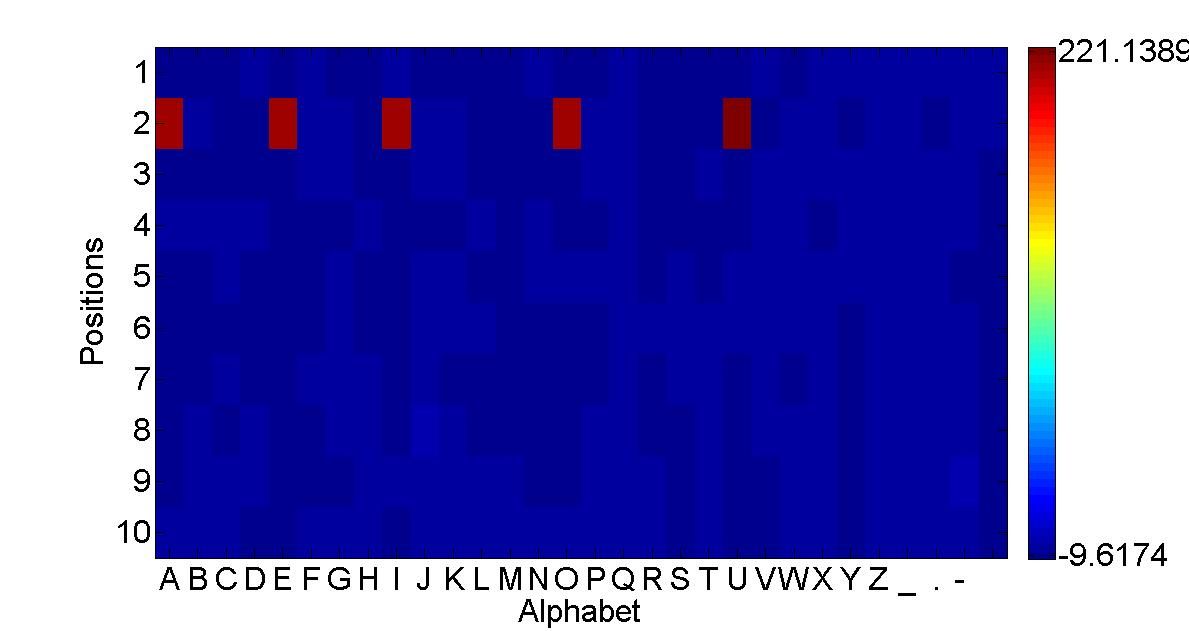
\includegraphics[width=0.8\textwidth]{LearnBadges}
	\caption{Learning Badges Perfect Case}
\end{figure}

\noindent For the second part, the position is changed to 5:10. The accuracyInTrain$=1$, and accuracyInTest$=0.5851$. Compare Fig. 3 and Fig. 2 we can see that in the imperfect case, the weight is dispersed at many positions and many letters. This could be one implication that the resulting separator is not the correct one, which only fits the training data. From this we know that the hypothesis space is critical. 
\begin{figure}[h!]
	\centering
	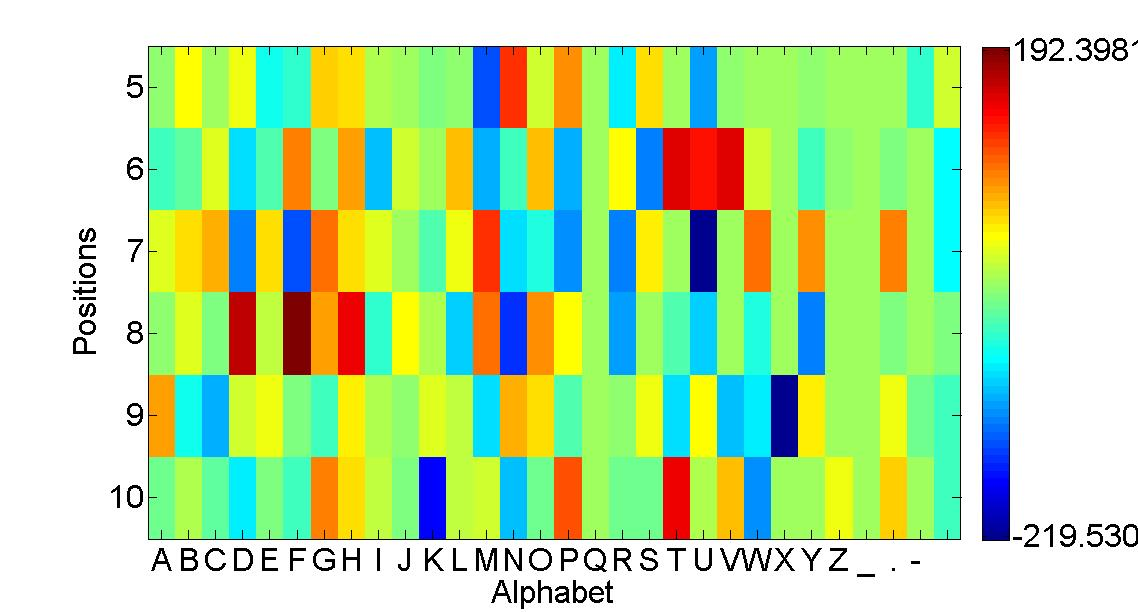
\includegraphics[width=0.8\textwidth]{LearBadges2}
	\caption{Learning Badges Imperfect Case}
\end{figure}


\subsubsection{Learning hyperplane}
\begin{figure}[h!]
	\centering
	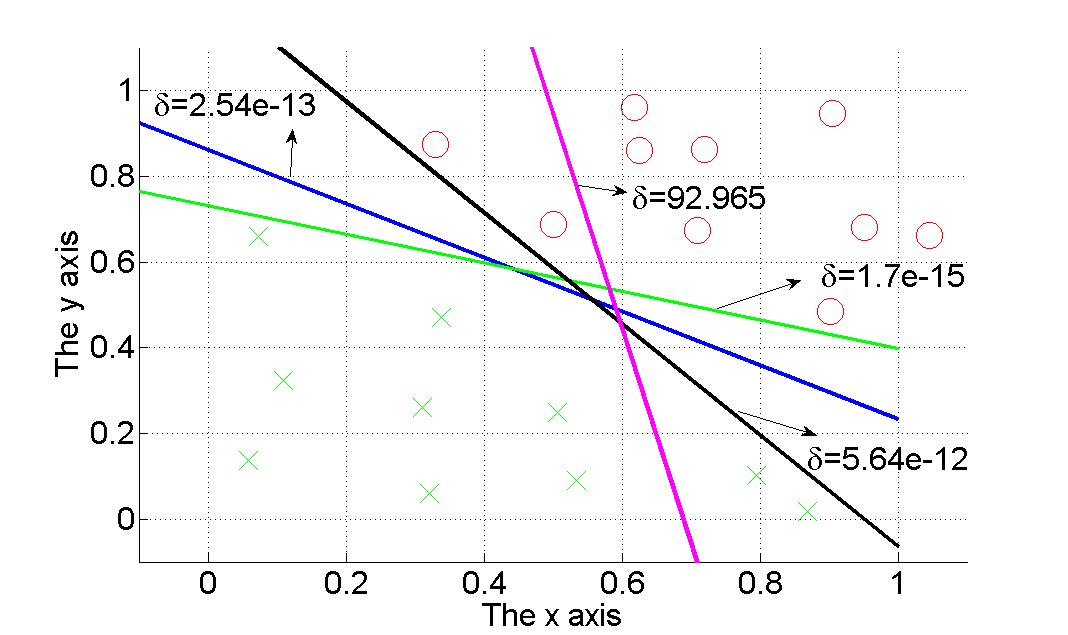
\includegraphics[width=0.8\textwidth]{LearnHyperPlane}
	\caption{Learning HyperPlane. $\delta$ of each plane is marked in the figure}
\end{figure}
\noindent From the figure we can see that the green, blue, and black plane separate the data exactly. Their corresponding $\delta$ is marked in the figure. From the linear program configuration, we know that if $\delta=0$, the resulting linear plane perfectly separates the data. In the numerical case, a ridiculously small $\delta$ basically means $\delta=0$. Note that the purple plane has $\delta=92.965$, so that the resulting plane does not separates the data.

\noindent I prefer to use the blue plane, because in the figure we can see that the minimum distance between the blue plane and the two dataset are bigger than the other two planes which also separate the data. From these examples we could infer that the solution to the linear program ([(2) to (4)]) is not unique. In fact it should have infinite number of solutions. Intuitively we could think of infinite number of parallel planes which are extremely close to a plane that separates two dataset. 

\end{document}

